\documentclass[11pt]{article}
% ============================================================
%  Policy Logic Forge -- technical report style
% ------------------------------------------------------------
%  Type   Libertinus Serif for prose, IBM Plex Sans for every
%         structural element (heads, labels, captions, figure
%         text), IBM Plex Mono for identifiers.  A humanist
%         serif carrying the argument with a technical grotesque
%         carrying the scaffolding: it should read as an
%         engineering report, not a paper template.
%  Colour Neutrals are biased toward the teal accent rather than
%         being pure greys, so the palette resolves as one set.
% ============================================================

\usepackage[letterpaper,top=1.05in,bottom=1.05in,left=1.15in,right=1.15in]{geometry}
\usepackage{libertinus-otf}
\usepackage{fontspec}
\usepackage[english]{babel}
\usepackage{microtype}
\usepackage{xcolor}
\usepackage{tikz}
\usetikzlibrary{arrows.meta,positioning,shapes.geometric,fit,backgrounds,calc,
                decorations.pathreplacing}
\usepackage{pgfplots}
\pgfplotsset{compat=1.18}
\usepackage{booktabs}
\usepackage{array}
\usepackage{longtable}
\usepackage{tabularx}
\usepackage{caption}
\usepackage{enumitem}
\usepackage{titlesec}
\usepackage{fancyhdr}
\usepackage{tcolorbox}
\tcbuselibrary{skins,breakable}
\usepackage[hidelinks]{hyperref}

% ---------------------------------------------------------------- palette
\definecolor{inkwell}{HTML}{14243A}   % body + heads
\definecolor{forge}{HTML}{0B6E75}     % primary accent
\definecolor{forgelight}{HTML}{D6E8E9}
\definecolor{slate}{HTML}{64748B}     % secondary text
\definecolor{amberdeep}{HTML}{A45309} % review / gate
\definecolor{amberpale}{HTML}{FBF0DF}
\definecolor{rosedeep}{HTML}{A3123A}  % stop / refusal
\definecolor{rosepale}{HTML}{FBE7EC}
\definecolor{mossdeep}{HTML}{14652F}  % pass / proved
\definecolor{mosspale}{HTML}{E4F1E6}
\definecolor{mist}{HTML}{F1F5F4}      % panel fill
\definecolor{hairline}{HTML}{C8D4D5}

% ---------------------------------------------------------------- fonts
\newfontfamily\plexsans{IBMPlexSans}[
  Extension=.otf, UprightFont=*-Regular, BoldFont=*-SemiBold,
  ItalicFont=*-Italic, BoldItalicFont=*-SemiBoldItalic,
  Ligatures=TeX, Scale=MatchLowercase]
\newfontfamily\plexsanslight{IBMPlexSans}[
  Extension=.otf, UprightFont=*-Light, BoldFont=*-Regular,
  Ligatures=TeX, Scale=MatchLowercase]
\newfontfamily\plexmono{IBMPlexMono}[
  Extension=.otf, UprightFont=*-Regular, BoldFont=*-SemiBold,
  ItalicFont=*-Italic, Ligatures=TeX, Scale=MatchLowercase]

\newcommand{\lbl}[1]{{\plexsans\bfseries\footnotesize\textcolor{forge}{\MakeUppercase{#1}}}}
\newcommand{\code}[1]{{\plexmono #1}}
\newcommand{\stage}[1]{{\plexmono\textcolor{inkwell}{#1}}}

\color{inkwell}

% ---------------------------------------------------------------- headings
\titleformat{\section}
  {\plexsans\bfseries\Large\color{inkwell}}
  {\textcolor{forge}{\thesection}}{0.7em}{}
  [\vspace{2pt}{\color{forge}\titlerule[1.2pt]}]
\titlespacing*{\section}{0pt}{2.4em plus .4em minus .2em}{1.1em}

\titleformat{\subsection}
  {\plexsans\bfseries\large\color{inkwell}}
  {\textcolor{forge}{\thesubsection}}{0.6em}{}
\titlespacing*{\subsection}{0pt}{1.7em plus .3em minus .2em}{0.6em}

\titleformat{\subsubsection}
  {\plexsans\bfseries\normalsize\color{slate}}
  {}{0pt}{}
\titlespacing*{\subsubsection}{0pt}{1.2em plus .2em}{0.4em}

% ---------------------------------------------------------------- captions
\captionsetup{
  font={small,color=slate},
  labelfont={color=forge},
  labelsep=period,
  justification=raggedright,
  singlelinecheck=false,
  skip=7pt}
\renewcommand{\figurename}{\textsc{Figure}}
\renewcommand{\tablename}{\textsc{Table}}

% ---------------------------------------------------------------- running heads
\pagestyle{fancy}
\fancyhf{}
\renewcommand{\headrulewidth}{0.4pt}
\renewcommand{\headrule}{\hbox to\headwidth{\color{hairline}\leaders\hrule height \headrulewidth\hfill}}
\fancyhead[L]{\plexsans\scriptsize\textcolor{slate}{\MakeUppercase{Policy Logic Forge}}}
\fancyhead[R]{\plexsans\scriptsize\textcolor{slate}{\nouppercase{\leftmark}}}
\fancyfoot[C]{\plexsans\small\textcolor{slate}{\thepage}}
\renewcommand{\sectionmark}[1]{\markboth{#1}{}}

% ---------------------------------------------------------------- tables
\renewcommand{\arraystretch}{1.28}
\newcolumntype{L}[1]{>{\raggedright\arraybackslash}p{#1}}
\newcolumntype{C}[1]{>{\centering\arraybackslash}p{#1}}
\newcommand{\thead}[1]{{\plexsans\bfseries\small\textcolor{forge}{#1}}}

% ---------------------------------------------------------------- callouts
\newtcolorbox{keypoint}[1][]{
  enhanced, breakable, sharp corners,
  colback=mist, colbacktitle=mist, colframe=forge,
  boxrule=0pt, leftrule=2.5pt,
  left=11pt, right=11pt, top=9pt, bottom=9pt,
  fonttitle=\plexsans\bfseries\small,
  coltitle=forge, #1}

\newtcolorbox{caution}[1][]{
  enhanced, breakable, sharp corners,
  colback=amberpale, colbacktitle=amberpale, colframe=amberdeep,
  boxrule=0pt, leftrule=2.5pt,
  left=11pt, right=11pt, top=9pt, bottom=9pt,
  fonttitle=\plexsans\bfseries\small,
  coltitle=amberdeep, #1}

\newtcolorbox{negative}[1][]{
  enhanced, breakable, sharp corners,
  colback=rosepale, colbacktitle=rosepale, colframe=rosedeep,
  boxrule=0pt, leftrule=2.5pt,
  left=11pt, right=11pt, top=9pt, bottom=9pt,
  fonttitle=\plexsans\bfseries\small,
  coltitle=rosedeep, #1}

% ---------------------------------------------------------------- lists
\setlist[itemize]{leftmargin=1.25em,itemsep=3pt,topsep=5pt,parsep=0pt}
\setlist[enumerate]{leftmargin=1.5em,itemsep=3pt,topsep=5pt,parsep=0pt}

% ---------------------------------------------------------------- tikz styles
\tikzset{
  node distance=7mm and 9mm,
  box/.style={
    draw=hairline, fill=white, rounded corners=2pt, line width=.7pt,
    inner sep=5pt, align=center, font=\plexsans\scriptsize,
    text=inkwell, minimum height=8mm},
  src/.style={box, fill=forgelight, draw=forge},
  gate/.style={box, fill=amberpale, draw=amberdeep, line width=1pt},
  stop/.style={box, fill=rosepale, draw=rosedeep},
  pass/.style={box, fill=mosspale, draw=mossdeep},
  hub/.style={box, fill=mist, draw=forge, line width=1.1pt},
  flow/.style={-{Stealth[length=2.2mm,width=1.6mm]}, draw=slate, line width=.7pt},
  backflow/.style={-{Stealth[length=2.2mm,width=1.6mm]}, draw=forge,
                   line width=1.1pt, dashed},
  phaseband/.style={rounded corners=3pt, draw=none, fill=mist},
  phaselabel/.style={font=\plexsans\bfseries\scriptsize, text=forge},
  edgelabel/.style={font=\plexsans\scriptsize, text=slate, inner sep=2pt,
                    fill=white, rounded corners=1pt},
}

\pgfplotsset{
  reportaxis/.style={
    width=\linewidth, height=6.2cm,
    axis line style={draw=hairline},
    tick label style={font=\plexsans\scriptsize, text=slate},
    label style={font=\plexsans\small, text=inkwell},
    title style={font=\plexsans\bfseries\small, text=inkwell},
    legend style={font=\plexsans\scriptsize, draw=hairline, fill=white},
    grid=major, grid style={draw=hairline, dashed, line width=.4pt},
    tick align=outside, tickpos=left,
  }
}

\newcommand{\rcCoverage}{11.8}
\newcommand{\rcRefusalRisk}{16.7}
\newcommand{\rcAnswerAllRisk}{12.1}
\newcommand{\rcN}{306}

\newcommand{\ladderStatute}{(0.0,0) (0.0,1) (0.0,2)}
\newcommand{\ladderPrivacy}{(2.5,0) (28.3,1) (63.6,2)}
\newcommand{\ladderNames}{raw,normalised,repaired}

\newcommand{\codesizecoords}{(15392,0) (10790,1) (1152,2) (15654,3)}
\newcommand{\locagents}{15,392}
\newcommand{\filesagents}{14}
\newcommand{\locutils}{10,790}
\newcommand{\filesutils}{32}
\newcommand{\loccli}{1,152}
\newcommand{\filescli}{3}
\newcommand{\loctests}{15,654}
\newcommand{\filestests}{64}
\newcommand{\loctotal}{42,988}


\hypersetup{
  pdftitle={Policy Logic Forge: A Technical Report},
  pdfauthor={Reza Rahimi},
  pdfsubject={Architecture of an evidence-carrying policy-to-logic pipeline}}

\begin{document}

% ================================================================ title
\begin{titlepage}
\thispagestyle{empty}
\noindent{\color{forge}\rule{\linewidth}{2.4pt}}

\vspace{2.2cm}
\noindent{\plexsans\bfseries\fontsize{15}{18}\selectfont\color{forge}
  POLICY LOGIC FORGE}

\vspace{0.9cm}
\noindent{\plexsanslight\fontsize{34}{40}\selectfont\color{inkwell}
  Turning regulation into\\
  logic you can check.}

\vspace{1.0cm}
\noindent{\itshape\fontsize{13.5}{18}\selectfont\color{slate}\raggedright
  A technical report on the architecture of an evidence-carrying pipeline
  that converts policy documents into business rules, decision and process
  models, information schemas, and a proof-checked intermediate
  representation --- deciding deterministically where it can, proving where
  a proof is possible, and refusing where the source does not support an
  answer.}

\vfill

\noindent\begin{minipage}[t]{0.48\linewidth}
  \lbl{author}\\[3pt]
  {\plexsans Reza Rahimi}
\end{minipage}\hfill
\begin{minipage}[t]{0.48\linewidth}
  \lbl{repository}\\[3pt]
  {\plexmono\small rrahimi-uci/policy-logic-forge}
\end{minipage}

\vspace{0.8cm}
\noindent\begin{minipage}[t]{0.48\linewidth}
  \lbl{document}\\[3pt]
  {\plexsans Architecture \& evaluation}
\end{minipage}\hfill
\begin{minipage}[t]{0.48\linewidth}
  \lbl{scope note}\\[3pt]
  {\plexsanslight\small\color{slate} This report describes what the system
   does and what it does not claim. It makes no assertion of legal
   correctness.}
\end{minipage}

\vspace{1.2cm}
\noindent{\color{hairline}\rule{\linewidth}{0.6pt}}
\end{titlepage}

% ================================================================ abstract
\section*{\plexsans Summary}
\addcontentsline{toc}{section}{Summary}
\vspace{-0.4em}
\noindent{\color{forge}\rule{\linewidth}{1.2pt}}
\vspace{0.8em}

\noindent
Most business systems do not implement a policy. They implement someone's
interpretation of a policy. A subject-matter expert identifies an
obligation, an analyst rewrites it as a requirement, an architect turns it
into a model, a developer writes the code, and an auditor later tries to
reconstruct why the system behaved as it did. At every handoff a trigger,
an exception, or a scope qualifier can quietly disappear, and nothing in
the chain records that it has.

This report describes a pipeline built around a single ordering principle:
\emph{decide as much as possible with code, prove what can be proved, ask a
model only what genuinely requires judgment, and send a human only what
survives all three.} That ordering inverts the usual instinct of reaching
for a model first and adding guardrails afterwards. Here the model is the
last resort before a person, and every stage exists to make its job
smaller.

Three properties distinguish the design. Every emitted artifact resolves
back to the sentence it came from, and the verifying stage rebuilds that
evidence from the raw corpus rather than trusting the citation a rule
carries --- so a hallucinated citation cannot pass. A frozen intermediate
representation carries a formal semantics, and obligations such as
decision-table disjointness are \emph{proved} by exhaustive enumeration or
returned as \code{unknown}, never assessed. And the system refuses: where
the source does not support a construct, it declines to emit one and
records a typed reason.

The final sections report what the evaluation actually found, including a
pre-registered hypothesis that failed. A companion experiment tested
whether the pipeline's own refusals predict where a language model errs.
They do not --- and the derived selector performs worse than answering
everything. That result is reported here in full, because a report that
only carries its successes is not evidence of anything.

\vspace{1.2em}
\noindent{\color{hairline}\rule{\linewidth}{0.6pt}}

\clearpage
\tableofcontents
\clearpage

% ================================================================ 1
\section{The translation gap}

A policy is not an algorithm. It is prose written to be read by a person
who will supply context, resolve ambiguity, and know which exceptions
matter. Turning it into something a machine executes requires answering
questions the prose never states explicitly:

\begin{itemize}
  \item Who is the responsible actor, and who is merely mentioned?
  \item What event triggers the obligation, and when does it lapse?
  \item Which conditions are cumulative, and which are alternatives?
  \item What is the scope --- which jurisdictions, parties, categories?
  \item Which sentence licenses each of the above?
\end{itemize}

Answering those is interpretation, and interpretation is where meaning
gets lost. The failure mode that matters is not output that looks wrong.
It is output that looks right: a well-formed decision table, correctly
typed, elegantly rendered, resting on a condition nobody in the source
document ever wrote.

\begin{keypoint}[title={The design constraint}]
A system that generates policy logic must be able to answer, for any
element it produces, \emph{which sentence licensed this} --- and that
answer must be checkable by something other than the component that
produced it.
\end{keypoint}

\subsection{Four kinds of check}

The architecture rests on an ordering of verification instruments by
strength. Every question is pushed down to the strongest instrument that
can settle it; only what no instrument can settle reaches a person.

\begin{figure}[htbp]
  \centering
  \resizebox{\linewidth}{!}{% Four kinds of check, in order of strength. Every question is pushed down
% to the strongest instrument that can settle it; only what survives all
% four reaches a person.
\begin{tikzpicture}[font=\plexsans\scriptsize, y=-1.62cm]

  \tikzset{rung/.style={box, text width=12.4cm, minimum height=1.34cm,
                        align=left, inner sep=8pt}}

  \node[rung, pass]  (r1) at (0,0) {%
    \lbl{1 · deterministic · no model}\\[3pt]
    \textbf{Decided by code, reproducible by anyone.}
    {\plexsanslight Does the quote occur in the cited chunk?\ ·\ Does this
     rule id exist?\ ·\ Does the schema hold?\ ·\ Does B read what A assigns?}};

  \node[rung, src]   (r2) at (0,1) {%
    \lbl{2 · proof · bounded, sound, incomplete by design}\\[3pt]
    \textbf{Proved exhaustively --- or returned as \code{unknown}.}
    {\plexsanslight Does this \code{UNIQUE} table satisfy pairwise
     disjointness?\ ·\ Is this condition satisfiable at all?}};

  \node[rung]        (r3) at (0,2) {%
    \lbl{3 · model · only where judgment is irreducible}\\[3pt]
    \textbf{Judged against fresh evidence, never the prior answer.}
    {\plexsanslight Does this description faithfully state the obligation?
     Evidence is rebuilt from the raw corpus, so errors do not correlate.}};

  \node[rung, gate]  (r4) at (0,3) {%
    \lbl{4 · human expert · routed, not replaced}\\[3pt]
    \textbf{Is this a correct reading of the regulation?}
    {\plexsanslight The one question no check above can answer --- which is
     why it should not be spent on the ones they can.}};

  \foreach \a/\b in {r1/r2, r2/r3, r3/r4}
    \draw[flow] (\a.south) -- (\b.north);

  % strength axis
  \draw[draw=hairline, line width=.8pt]
        ($(r1.north west)+(-0.30,0)$) -- ($(r4.south west)+(-0.30,0)$);
  \node[rotate=90, anchor=south, font=\plexsans\tiny, text=slate]
        at ($(r1.west)!0.5!(r4.west)+(-0.42,0)$)
        {decreasing strength\ \ ·\ \ increasing cost};

\end{tikzpicture}
}
  \caption{The verification ladder. Most questions a policy pipeline must
    answer are not matters of opinion --- whether a quoted sentence occurs
    in the cited chunk is string resolution, whether a rule identifier
    exists is set membership, whether rule~B reads what rule~A assigns is a
    dataflow test. The difference this design makes is not a better judge;
    it is far fewer questions that need judging.}
  \label{fig:ladder}
\end{figure}

The economic argument follows from the ordering. Expert review is the
genuine gold standard for legal correctness and cannot be replaced --- but
an expert cannot read several hundred rules by hand every time a policy
changes. Spending that attention on questions a string comparison could
have settled is the waste the ladder exists to eliminate.

% ================================================================ 2
\section{Pipeline architecture}

The system runs thirteen stages in order. The stage number and the agent
identifier are always the same value, so \code{-{}-stage 9} and
\code{-{}-agent agent\_09} select the same stage. Each stage is a
subprocess that checkpoints its output, so a run can resume from any
boundary.

\begin{figure}[htbp]
  \centering
  \resizebox{\linewidth}{!}{% Thirteen stages, grouped by the responsibility each boundary carries.
% Nodes are placed on an integer grid; the phase bands are then FITTED to
% the nodes they contain on a background layer, so no height or offset is
% ever computed by hand and a band can never drift from its contents.
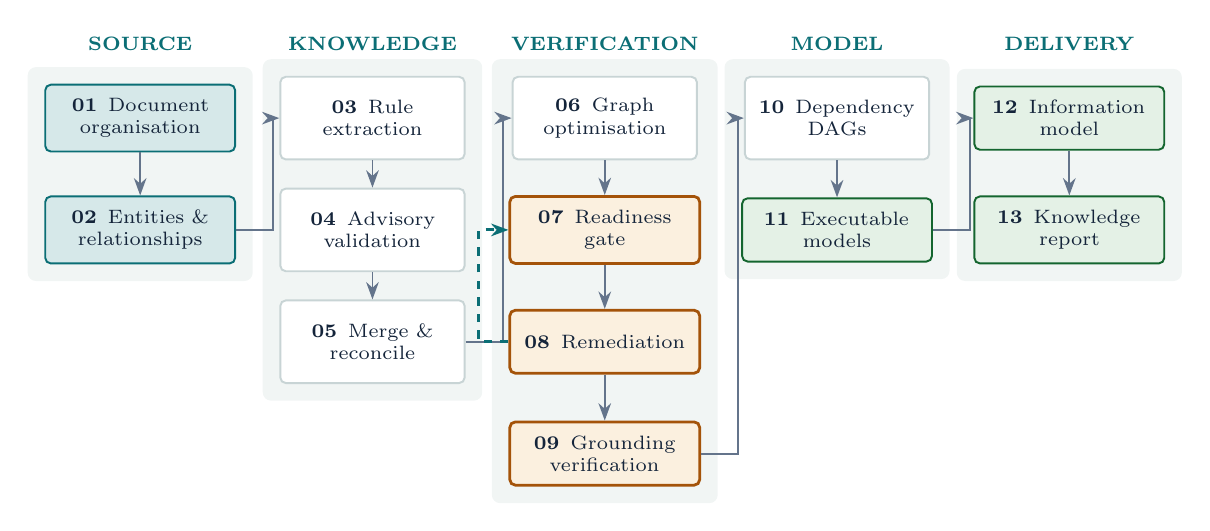
\begin{tikzpicture}[font=\plexsans\scriptsize, x=2.95cm, y=-1.42cm]

  \tikzset{st/.style={box, text width=2.06cm, minimum height=1.05cm,
                      inner sep=4pt}}

  % ---- stages, by (column = phase, row) --------------------------------
  \node[st, src]  (s1)  at (0,0) {\textbf{01}\enspace Document\\organisation};
  \node[st, src]  (s2)  at (0,1) {\textbf{02}\enspace Entities \&\\relationships};

  \node[st]       (s3)  at (1,0) {\textbf{03}\enspace Rule\\extraction};
  \node[st]       (s4)  at (1,1) {\textbf{04}\enspace Advisory\\validation};
  \node[st]       (s5)  at (1,2) {\textbf{05}\enspace Merge \&\\reconcile};

  \node[st]       (s6)  at (2,0) {\textbf{06}\enspace Graph\\optimisation};
  \node[st, gate] (s7)  at (2,1) {\textbf{07}\enspace Readiness\\gate};
  \node[st, gate] (s8)  at (2,2) {\textbf{08}\enspace Remediation};
  \node[st, gate] (s9)  at (2,3) {\textbf{09}\enspace Grounding\\verification};

  \node[st]       (s10) at (3,0) {\textbf{10}\enspace Dependency\\DAGs};
  \node[st, pass] (s11) at (3,1) {\textbf{11}\enspace Executable\\models};

  \node[st, pass] (s12) at (4,0) {\textbf{12}\enspace Information\\model};
  \node[st, pass] (s13) at (4,1) {\textbf{13}\enspace Knowledge\\report};

  % ---- phase bands, fitted to their contents ---------------------------
  \begin{scope}[on background layer]
    \node[phaseband, fit=(s1)(s2),                inner sep=6pt] (b0) {};
    \node[phaseband, fit=(s3)(s4)(s5),            inner sep=6pt] (b1) {};
    \node[phaseband, fit=(s6)(s7)(s8)(s9),        inner sep=6pt] (b2) {};
    \node[phaseband, fit=(s10)(s11),              inner sep=6pt] (b3) {};
    \node[phaseband, fit=(s12)(s13),              inner sep=6pt] (b4) {};
  \end{scope}

  % all five labels share one baseline, set from the tallest band
  \foreach \c/\name in {0/SOURCE, 1/KNOWLEDGE, 2/VERIFICATION,
                        3/MODEL, 4/DELIVERY}
    \node[phaselabel, anchor=south] at (\c, -0.52) {\name};

  % ---- flow within a phase ---------------------------------------------
  \foreach \a/\b in {s1/s2, s3/s4, s4/s5, s6/s7, s7/s8, s8/s9, s10/s11, s12/s13}
    \draw[flow] (\a) -- (\b);

  % ---- hand-off between phases (always from the last stage of a phase) --
  \draw[flow] (s2.east)  -- ++(0.16,0) |- (s3.west);
  \draw[flow] (s5.east)  -- ++(0.16,0) |- (s6.west);
  \draw[flow] (s9.east)  -- ++(0.16,0) |- (s10.west);
  \draw[flow] (s11.east) -- ++(0.16,0) |- (s12.west);

  % ---- remediation loop: 08 re-enters the gate at 07 -------------------
  % Routed down the left gutter, which is empty; the right of this column
  % carries the 09 -> 10 hand-off. No inline label -- at this scale it can
  % only be set on top of stage 04, so the caption carries the meaning.
  \draw[backflow] (s8.west) -- ++(-0.13,0) |- (s7.west);

\end{tikzpicture}
}
  \caption{The thirteen stages, grouped by the responsibility each boundary
    carries. Amber stages form the verification block and share one
    directory because they read and write the same optimised graph. The
    dashed edge is the remediation loop: stage~08 patches only the fields
    that failed and re-enters the gate at stage~07, never re-extracting.}
  \label{fig:pipeline}
\end{figure}

\begin{table}[htbp]
\centering
\caption{Stage responsibilities and primary outputs.}
\label{tab:stages}
{\small
\begin{tabularx}{\linewidth}{@{}p{0.055\linewidth} p{0.30\linewidth} X@{}}
\toprule
\thead{Stage} & \thead{Responsibility} & \thead{Primary output} \\
\midrule
01 & Document organisation      & \code{agent\_01-organized-documents/} \\
02 & Entity and relationship extraction & \code{agent\_02-entities/} \\
03 & Business-rule extraction   & \code{agent\_03-rules/} \\
04 & Advisory rule validation   & \code{agent\_04-validation/} (consumed by nothing; advisory by design) \\
05 & Rules/entities merge       & first complete knowledge graph \\
06 & Graph optimisation         & dedup + dependency analysis \\
07 & Executable-readiness gate  & readiness report; four invariants \\
08 & Readiness remediation      & focused field patches, only if 07 requests them \\
09 & Grounding verification     & claim-level certification \\
10 & Dependency-DAG generation  & \code{dependency\_dags.json}, 100\,\% coverage \\
11 & Executable model generation & DMN, BPMN, CMMN, SBVR + LExec compile \\
12 & Business information model & LinkML schema, classes, typed attributes \\
13 & Business knowledge report  & self-contained HTML, zero network calls \\
\bottomrule
\end{tabularx}}
\end{table}

\subsection{The evidence spine}

Every artifact resolves back to the sentence it came from, and every step
of that walk is checked rather than asserted. This is the single property
the rest of the design exists to protect.

Traceability alone is cheap: any system can store a pointer alongside a
generated rule, and a pointer that was never checked is exactly as
convincing as one that was. What makes the spine load-bearing is the
direction of the arrows. The forward path carries meaning from a passage
into a rule, a symbol, an attribute, and finally into a decision table or a
schema. The return path re-derives that evidence \emph{independently},
from the raw corpus, using none of the intermediate structure the forward
path built.

That asymmetry is what a hallucinated citation cannot survive. A rule
asserting support from a sentence that does not exist will resolve forward
perfectly well --- the artifact renders, the types check, the table is
well-formed --- and fail only when something goes back to the document and
looks.

\begin{figure}[htbp]
  \centering
  \resizebox{\linewidth}{!}{% The evidence spine. The reverse arrow along the bottom is the one that
% matters: agent_09 does not trust a stored citation, it rebuilds the
% evidence from the raw corpus, so a hallucinated citation cannot pass.
%
% Edge labels are deliberately placed BELOW their arrows on the long
% horizontal runs only. On short runs there is no room for a label that
% does not sit on a box, so those carry none and the caption explains.
\begin{tikzpicture}[font=\plexsans\scriptsize, x=3.30cm, y=-1.70cm]

  \tikzset{sp/.style={box, text width=2.15cm, minimum height=1.20cm}}

  % --- the chain -------------------------------------------------------
  \node[sp, src]  (doc)  at (0,0) {\textbf{Source passage}\\[1pt]
                                   {\plexsanslight chunk + section}};
  \node[sp]       (rule) at (1,0) {\textbf{Rule}\\[1pt]
                                   {\plexsanslight typed conditions\\and outcomes}};
  \node[sp]       (sym)  at (2,0) {\textbf{Symbol}\\[1pt]
                                   {\plexsanslight unit, value set,\\range}};
  \node[sp, pass] (attr) at (3,0) {\textbf{Attribute}\\[1pt]
                                   {\plexsanslight on a class}};

  % No inline edge labels: the gaps between these boxes are narrower than
  % any label that would go in them, so a label here can only be set on top
  % of a box. The caption names the stage that performs each step instead.
  \foreach \a/\b in {doc/rule, rule/sym, sym/attr}
    \draw[flow] (\a) -- (\b);

  % --- the gates that sit on the chain ---------------------------------
  \node[sp, gate] (g1) at (1,1.15) {\code{agent\_07}\\[1pt]
                                    {\plexsanslight four invariants}};
  \node[sp, gate] (g2) at (2,1.15) {\code{agent\_09}\\[1pt]
                                    {\plexsanslight claim-level\\certification}};
  \draw[draw=amberdeep, line width=.9pt] (rule) -- (g1);
  \draw[draw=amberdeep, line width=.9pt] (sym)  -- (g2);

  % --- what the chain produces -----------------------------------------
  \node[sp, pass] (model)  at (3,1.15) {\textbf{DMN · BPMN}\\\textbf{CMMN · SBVR}\\
                                        {\plexsanslight LinkML}};
  \node[sp, pass] (report) at (3,2.30) {\textbf{Report row}};

  \draw[flow] (attr)  -- (model);
  \draw[flow] (model) -- (report);
  \draw[flow] (rule.north) -- ++(0,-0.34) -| (model.north);

  % --- the reverse arrow: the property the whole design protects --------
  \draw[backflow] (g2.south) -- ++(0,0.62) -| (doc.south);
  \node[edgelabel, font=\plexsans\tiny, text=forge]
        at (1.0,1.92) {evidence rebuilt from the raw corpus, not from the citation};

\end{tikzpicture}
}
  \caption{The evidence spine. Stage~03 extracts rules from source
    passages; stage~12 types symbols into class attributes. The dashed
    return path is the one that matters: stage~09 does not trust the
    citation a rule carries, it rebuilds the evidence from the raw corpus.
    On one real run that pass rejected \textbf{44\,\%} of the dependency and
    conflict claims the pipeline's own deterministic guard had already
    accepted.}
  \label{fig:spine}
\end{figure}

% ================================================================ 3
\section{Orchestration}

A stage is a subprocess, so its exit code is the only signal the
orchestrator can route on. There are three meanings, and one is
deliberately overloaded.

\begin{figure}[htbp]
  \centering
  \resizebox{0.96\linewidth}{!}{% The exit-code contract. A stage is a subprocess, so its exit code is the
% only thing the orchestrator can route on -- and code 3 is overloaded,
% which is why it branches again on the stage that produced it.
%
% Column spacing must exceed the widest box or the columns collide; the
% x unit below is set from the box width, not guessed.
\begin{tikzpicture}[font=\plexsans\scriptsize, x=4.45cm, y=-1.16cm]

  \tikzset{
    ec/.style={box, text width=3.15cm, minimum height=1.00cm},
    dec/.style={box, fill=mist, draw=slate, text width=1.35cm,
                minimum height=0.86cm},
    term/.style={box, rounded corners=8pt, text width=1.35cm,
                 minimum height=0.72cm, font=\plexsans\bfseries\scriptsize}}

  \node[dec] (c) at (0,2) {exit code};

  \node[ec, pass] (ok)    at (1,0) {\textbf{0}\enspace Work done,\\nothing to flag};
  \node[dec]      (w)     at (1,1.6) {\textbf{3}\\which stage?};
  \node[ec, stop] (miss)  at (1,3.1) {\textbf{2}\enspace Required upstream\\artifact missing};
  \node[ec, stop] (crash) at (1,4.3) {\textbf{1}\enspace Unhandled runtime\\or config error};

  \node[ec, gate] (qual) at (2,0.75) {\code{07 · 08 · 09 · 12}\\[1pt]
        \textbf{Data quality}\\{\plexsanslight output written, needs review}};
  \node[ec, stop] (part) at (2,2.55) {\code{03}\\[1pt]
        \textbf{Extraction incomplete}\\{\plexsanslight partials kept for resume}};

  \node[term, pass] (cont) at (3,0.0) {continue};
  \node[term, stop] (halt) at (3,3.6) {stop};

  \foreach \t in {ok, w, miss, crash} \draw[flow] (c) -- (\t);
  \draw[flow] (w) -- (qual);
  \draw[flow] (w) -- (part);
  \draw[flow] (ok)   -- (cont);
  \draw[flow] (qual) -- (cont);
  \foreach \s in {part, miss, crash} \draw[flow] (\s) -- (halt);

\end{tikzpicture}
}
  \caption{The exit-code contract. Code~3 branches on the stage that
    produced it: for the quality-gated stages it is a data-quality signal
    and the run continues carrying review flags, but for stage~03 it means
    extraction was incomplete and the run must stop so no later stage
    consumes a partial graph.}
  \label{fig:exitcodes}
\end{figure}

Two invariants follow, and both were violated in practice before they were
enforced:

\begin{itemize}
  \item \textbf{A stage may never exit 0 for work it did not do.}
    Stages~02 and~03 once printed ``No documents found'' and returned
    normally, so a run over an empty corpus was reported as successful
    through three further stages and only stopped at stage~05, blaming its
    own missing inputs.
  \item \textbf{A missing input is reported, not raised.} Stages~07, 08
    and~09 died on an unhandled \code{FileNotFoundError}, which exits~1 ---
    a code the orchestrator reads as a crash --- and printed a traceback
    that said nothing about which stage to run first.
\end{itemize}

\subsection{The readiness gate}

Stage~07 completes every rule's evidence-dependent fields through bounded
evidence retrieval over the full corpus, then validates the graph against
four deterministic invariants. Evidence retrieval builds an inverted token
index --- words, path tokens, and exception markers such as ``except'',
``unless'', ``notwithstanding'' --- \emph{before} any model call, so the
search record can prove the whole corpus was inspected.

\begin{table}[htbp]
\centering
\caption{The four readiness invariants.}
\label{tab:invariants}
{\small
\begin{tabularx}{\linewidth}{@{}p{0.24\linewidth} X@{}}
\toprule
\thead{Invariant} & \thead{What it checks} \\
\midrule
\code{corpus\_integrity} &
  Every cited-section addition or removal between the baseline and final
  graph carries an explicit reason string. \\
\code{naming\_consistency} &
  Zero entity-key violations against the canonical pattern
  \code{\^{}[A-Z][A-Z0-9]*(?:\_[A-Z0-9]+)*\$}. \\
\code{schema\_consistency} &
  Zero \emph{blocking} contract violations. Deliberately gated on blocking
  errors alone: folding in evidence and provenance gaps made this invariant
  fail on every run containing any review-required rule, pre-empting
  stage~08 before it could run. \\
\code{referential\_integrity} &
  Zero dependency edges pointing at a \code{rule\_id} that does not exist. \\
\bottomrule
\end{tabularx}}
\end{table}

\subsection{What ``independent'' verification means}

Stage~09 certifies each source-derived field claim by claim against text it
re-locates itself. Two design choices make it genuinely independent rather
than a second opinion from the same source:

\begin{itemize}
  \item Claims split into two \emph{disjoint} paths.
    \code{description}, \code{condition}, \code{outcome}, \code{party},
    \code{scope} and \code{exception} are model-verified against an
    evidence packet the stage rebuilds from the raw corpus.
    \code{condition\_logic} and \code{test\_vector} are excluded from model
    verification entirely --- they are pipeline-derived values, not
    sentences any document states verbatim, and asking a model for a
    literal quote scored near-100\,\% false-insufficient in practice. Those
    are checked structurally instead.
  \item Every verdict of \emph{supported} or \emph{contradicted} is
    downgraded to \emph{insufficient evidence} unless the model's cited
    quote resolves to a genuine substring of the real corpus text. A
    hallucinated citation cannot pass even when the model asserts support.
\end{itemize}

\begin{keypoint}[title={Coverage is not the same as outcome}]
\code{claim\_coverage\_percent} measures response-set \emph{completeness}
--- did the verifier return exactly one verdict per claim, none missing,
duplicated, or unexpected. It is a fail-closed integrity check on the
verification pipeline itself, and is deliberately distinct from the
supported/contradicted/insufficient counts. An incomplete verification run
is a hard stop, never silently accepted.
\end{keypoint}

% ================================================================ 4
\section{The compiler layer}

Alongside the review-oriented model outputs, the pipeline compiles the
subset of rules it can represent into \textbf{LExec}, an intermediate
representation with a frozen semantics. This path is additive and
best-effort: a compile failure never blocks or replaces the review
projection.

\begin{table}[htbp]
\centering
\caption{LExec IR semantics, v1.}
\label{tab:ir}
{\small
\begin{tabularx}{\linewidth}{@{}p{0.26\linewidth} X@{}}
\toprule
\thead{Property} & \thead{Commitment} \\
\midrule
Null model & Kleene three-valued logic \\
Table boundary & \code{unknown} at a table boundary means \emph{refuse}, not \emph{default} \\
Exception reading & defeater-or \\
Operators &
  \code{and or not is\_null eq ne lt le gt ge contains in\_binned\_range} \\
Effects & assignment only \\
Arithmetic & \textbf{none} --- the IR has no arithmetic at all \\
Numeric theory & v2 \code{number} always lowers to \code{real}; an integer
  theory is never inferred from an integral-looking value \\
\bottomrule
\end{tabularx}}
\end{table}

The absence of arithmetic is a deliberate scope boundary, and Section~\ref{sec:eval}
reports what it costs.

\subsection{Bounded proof, not a solver}

Proof obligations --- principally pairwise disjointness for \code{UNIQUE}
hit-policy tables --- are discharged by exhaustive enumeration over finite
domains, capped at $10{,}000$ assignments. The prover deliberately does not
pretend to be a complete SMT backend.

\begin{keypoint}[title={Sound, and incomplete on purpose}]
The prover returns \code{unsat} only when the enumeration was
\emph{complete}. If the domain is unbounded or the cap is reached it
returns \code{unknown} --- never a green tick it cannot justify. Soundness
is what is claimed; completeness is explicitly not.
\end{keypoint}

\subsection{Properties proved rather than tested}

A test checks that one example behaved. The properties below are checked
exhaustively over the bounded signature, so they hold for every input in
it, not for the ones a test author happened to choose. All six are
discharged by \code{proofs/check\_properties.py} in a couple of seconds.

\begin{table}[htbp]
\centering
\caption{Machine-checked properties. All hold.}
\label{tab:proofs}
{\small
\begin{tabularx}{\linewidth}{@{}p{0.035\linewidth} X p{0.26\linewidth}@{}}
\toprule
\thead{\#} & \thead{Property} & \thead{Method} \\
\midrule
1 & $(T, \sqsubset)$ is a strict partial order --- irreflexive, asymmetric,
    transitive & all 3{,}615 tuples \\
2 & \code{reconcile\_types}$(S)$ returns the unique $\sqsubset$-least
    element or $\bot$, never a coercion & all 1{,}940 subsets \\
3 & \textsc{Money} $\parallel$ \textsc{Percentage} --- neither refines the
    other & direct \\
4 & Prover soundness: $\mathrm{sat}(w) \Rightarrow w \models \varphi$ and
    $\mathrm{unsat} \Rightarrow \varphi$ unsatisfiable
  & 212 formulas $\times$ 48 assignments, 0 violations \\
5 & Decidability on a bounded signature & 0 unknowns, 0 disagreements with
    brute force \\
6 & The dependency DAG set is a partition of the rule set & checked on a
    real 832-rule run \\
\bottomrule
\end{tabularx}}
\end{table}

Property~3 is the legible one. \textsc{Money} and \textsc{Percentage} are
both decimal numbers, and a system that quietly reconciles them will
eventually read a 3\,\% rate as \$3. That cannot happen here, and
\emph{cannot} is the operative word: it is not a test that passed on the
inputs someone thought of, it is a property that holds for every pair of
types in the system.

Property~4 is the one that matters most for trust, because it is the
checker checking itself.

% ================================================================ 5
\section{Generated artifacts}

Stage~11 emits standards-aligned models. Generation is gated on source
support, not on whether a rule happens to have a dependency.

\begin{table}[htbp]
\centering
\caption{Output formats and the question each answers.}
\label{tab:formats}
{\small
\begin{tabularx}{\linewidth}{@{}p{0.13\linewidth} p{0.28\linewidth} X@{}}
\toprule
\thead{Format} & \thead{Question it answers} & \thead{Note} \\
\midrule
DMN 1.3   & What is decided, given these inputs? & Real emitter; hit policy carried through \\
BPMN 2.0  & In what order, by whom?              & Deliberately conservative --- see below \\
CMMN 1.1  & What may a knowledge worker do?      & Intentionally simple \\
SBVR      & What does the vocabulary mean?       & Project-aligned profile, \emph{not} full OMG interchange conformance \\
LinkML    & What is the data shape?              & Canonical form; JSON Schema and diagrams generated from it \\
LExec IR  & What can be proved?                  & Proof-checked side channel, additive \\
\bottomrule
\end{tabularx}}
\end{table}

\begin{keypoint}[title={The most useful thing the system does is refuse}]
BPMN generation requires an evidenced trigger, a responsible actor, and at
least two explicitly ordered steps in the source. On privacy policies that
test declines for the overwhelming majority of rules --- which is the
correct answer, not a shortfall, because a privacy policy states
obligations, it does not describe workflows. Generating a diagram for every
rule would have looked like far more progress and meant considerably less.
\end{keypoint}

\subsection{Module structure}

Most of \code{utils/} is used directly by one or more stages with no
interesting internal structure. The compiler layer is the exception: it is
a genuine hub.

\begin{figure}[htbp]
  \centering
  \resizebox{\linewidth}{!}{% The compiler layer is the only part of utils/ with real internal
% structure: lexec_ir.py is a genuine hub, imported both by the stage-11
% proof-checked compile path and by every RegDelta module.
%
% Module names are set in mono, which is wide. Box width is chosen from the
% longest name (impact_propagation, 18 characters), not guessed.
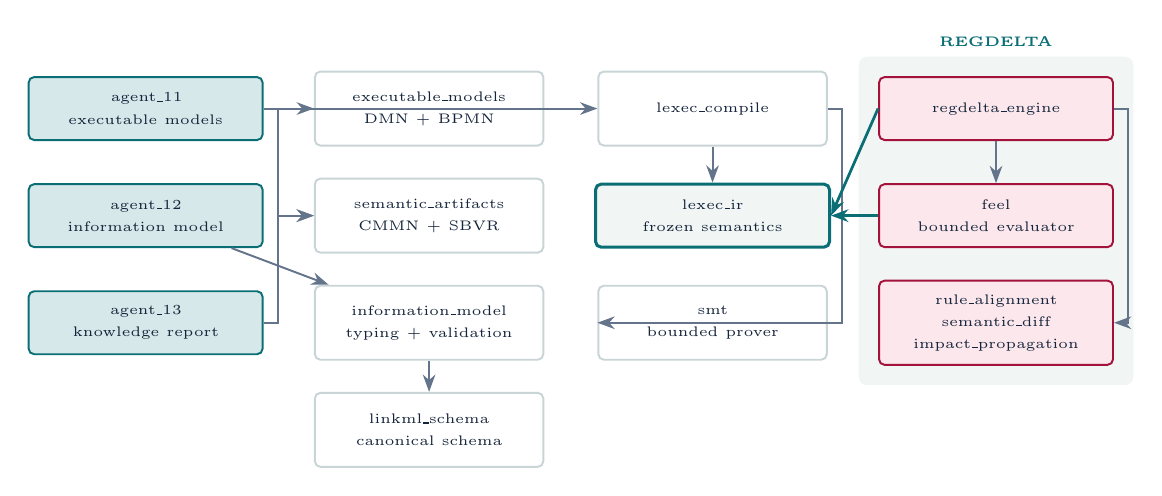
\begin{tikzpicture}[font=\plexsans\scriptsize, x=3.60cm, y=-1.36cm]

  \newcommand{\mname}[1]{{\plexmono\tiny #1}}
  \newcommand{\msub}[1]{{\plexsanslight\tiny #1}}
  \tikzset{m/.style={box, text width=2.62cm, minimum height=0.94cm,
                     inner sep=4pt}}

  % pipeline entry points
  \node[m, src] (a11) at (0,0) {\mname{agent\_11}\\\msub{executable models}};
  \node[m, src] (a12) at (0,1) {\mname{agent\_12}\\\msub{information model}};
  \node[m, src] (a13) at (0,2) {\mname{agent\_13}\\\msub{knowledge report}};

  % emitters and typing
  \node[m] (em) at (1,0) {\mname{executable\_models}\\\msub{DMN + BPMN}};
  \node[m] (sa) at (1,1) {\mname{semantic\_artifacts}\\\msub{CMMN + SBVR}};
  \node[m] (im) at (1,2) {\mname{information\_model}\\\msub{typing + validation}};
  \node[m] (lk) at (1,3) {\mname{linkml\_schema}\\\msub{canonical schema}};

  % proof-checked path
  \node[m]      (lc)  at (2,0) {\mname{lexec\_compile}};
  \node[m, hub] (ir)  at (2,1) {\mname{lexec\_ir}\\\msub{frozen semantics}};
  \node[m]      (smt) at (2,2) {\mname{smt}\\\msub{bounded prover}};

  % regdelta
  \node[m, stop] (re)   at (3,0) {\mname{regdelta\_engine}};
  \node[m, stop] (feel) at (3,1) {\mname{feel}\\\msub{bounded evaluator}};
  \node[m, stop] (rest) at (3,2) {\mname{rule\_alignment}\\\mname{semantic\_diff}\\%
                                  \mname{impact\_propagation}};

  \draw[flow] (a11) -- (em);
  \draw[flow] (a11.east) -- ++(0.05,0) |- (sa.west);
  \draw[flow] (a13.east) -- ++(0.05,0) |- (sa.west);
  \draw[flow] (a12) -- (im);
  \draw[flow] (im) -- (lk);
  \draw[flow] (a11.east) -- ++(0.05,0) |- (lc.west);
  \draw[flow] (lc) -- (ir);
  \draw[flow] (lc.east) -- ++(0.05,0) |- (smt.west);

  \draw[flow] (re) -- (feel);
  \draw[flow] (re.east) -- ++(0.05,0) |- (rest.east);
  \draw[flow, draw=forge, line width=1pt] (re.west)   -- (ir.east);
  \draw[flow, draw=forge, line width=1pt] (feel.west) -- (ir.east);

  \begin{scope}[on background layer]
    \node[phaseband, fit=(re)(feel)(rest), inner sep=7pt] (rd) {};
  \end{scope}
  \node[phaselabel, anchor=south, font=\plexsans\bfseries\tiny]
        at (rd.north) {REGDELTA};

\end{tikzpicture}
}
  \caption{The compiler layer. Two independent emitter paths are easy to
    conflate: \code{executable\_models} and \code{semantic\_artifacts}
    produce the real DMN, BPMN, CMMN and SBVR outputs in every run and
    never touch the compiler, while \code{lexec\_compile} produces a
    separate proof-checked IR for the representable subset. Teal edges mark
    \code{lexec\_ir} as the shared hub.}
  \label{fig:modules}
\end{figure}

\subsection{RegDelta}

Given two completed runs, RegDelta answers \emph{what changed, for whom,
and what else does it affect} --- without re-running extraction.

\begin{figure}[htbp]
  \centering
  \resizebox{\linewidth}{!}{% RegDelta: what changed, for whom, and what else it affects -- computed
% from two completed runs without re-running extraction.
\begin{tikzpicture}[font=\plexsans\scriptsize, x=2.60cm, y=-1.40cm]

  \tikzset{rg/.style={box, text width=1.85cm, minimum height=1.06cm}}

  \node[rg, src] (old) at (0,0) {\textbf{old run}\\{\plexsanslight optimised graph}};
  \node[rg, src] (new) at (0,1) {\textbf{new run}\\{\plexsanslight optimised graph}};

  \node[rg] (comp)  at (1,0.5) {\textbf{Compile}\\{\plexsanslight both to LExec IR}};
  \node[rg] (align) at (2,0.5) {\textbf{Align}\\{\plexsanslight exact ID today}};
  \node[rg] (class) at (3,0.5) {\textbf{Classify}\\{\plexsanslight added · removed\\changed · unchanged}};
  \node[rg] (prop)  at (4,0.5) {\textbf{Propagate}\\{\plexsanslight direct → potential\\→ recompute}};
  \node[rg] (rep)   at (5,0.5) {\textbf{Replay}\\{\plexsanslight old vs new\\outcome}};

  \node[box, fill=mist, draw=forge, line width=1pt, text width=11.0cm,
        minimum height=0.80cm, align=center]
        (out) at (2.5,2.05)
        {\code{regdelta-impact/1.0}\quad
         {\plexsanslight rule\_alignments · semantic\_changes · affected\_cases ·
          witnesses · downstream\_impacts · refusals}};

  \draw[flow] (old.east) -- ++(0.08,0) |- (comp.west);
  \draw[flow] (new.east) -- ++(0.08,0) |- (comp.west);
  \foreach \a/\b in {comp/align, align/class, class/prop, prop/rep}
    \draw[flow] (\a) -- (\b);
  \draw[flow] (rep.south) |- (out.east);

\end{tikzpicture}
}
  \caption{The differential-execution pipeline. Every rule in scope
    resolves to exactly one of \emph{changed}, \emph{unchanged},
    \emph{unresolved-review}, or \emph{refused-unsupported-construct};
    refused and review-held rules stay in the denominator of every reported
    metric, so nothing is silently dropped.}
  \label{fig:regdelta}
\end{figure}

Two design choices are easy to get wrong by assumption:

\begin{itemize}
  \item \textbf{Alignment is exact-identifier only today.} It implements
    the first rung of a five-rung ladder (exact ID $\to$ source-section
    signature $\to$ predicate structure $\to$ semantic similarity $\to$
    explicit review). Two independently re-extracted runs of the same
    document will not align well yet; a renamed rule reads as a removal
    plus an addition.
  \item \textbf{\emph{Potential} is narrative reachability, not proven
    dependency.} It walks stage~10's DAG edges, which are extraction
    judgments about narrative dependency, not shared dataflow symbols.
\end{itemize}

% ================================================================ 6
\section{Evaluation}
\label{sec:eval}

\subsection{Does it transfer off the domain it was built on?}

The compile rate --- how often an extracted rule lowers to the checkable IR
--- was only ever measured on privacy policies. A pilot measured the same
number on an open benchmark of statutory reasoning, reporting a
\emph{raw~$\to$ normalised~$\to$ repaired} ladder with typed refusal codes
so that a failure states its reason.

\begin{figure}[htbp]
  \centering
  \resizebox{\linewidth}{!}{% Compile-rate ladder: privacy policies against the tax statute, at each
% repair stage. Coordinates generated from research/pilot/results/.
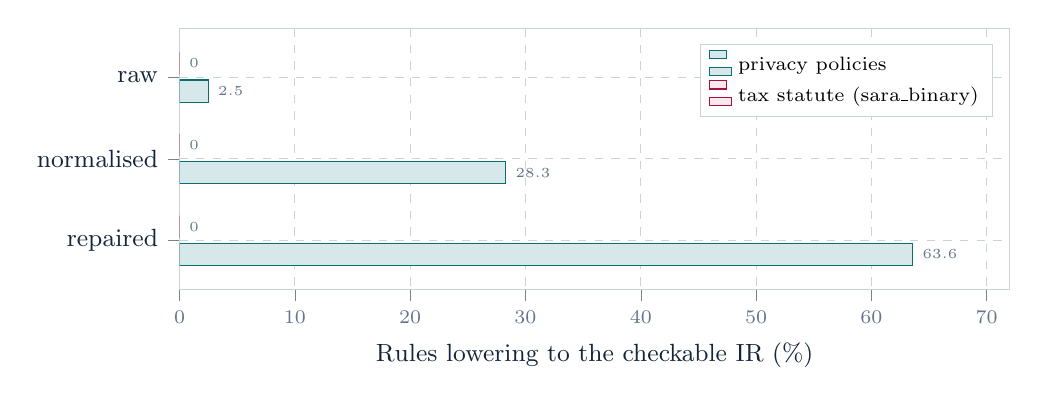
\begin{tikzpicture}
  \begin{axis}[reportaxis,
      height=4.9cm,
      xbar, y dir=reverse,
      xlabel={Rules lowering to the checkable IR (\%)},
      xmin=0, xmax=72,
      ytick={0,1,2},
      yticklabels={raw, normalised, repaired},
      y tick label style={font=\plexsans\small, text=inkwell},
      bar width=8pt,
      enlarge y limits=0.30,
      nodes near coords,
      nodes near coords style={font=\plexsans\tiny, text=slate,
                               /pgf/number format/fixed,
                               /pgf/number format/precision=1},
      legend style={at={(0.98,0.94)}, anchor=north east},
      legend cell align=left]

    \addplot[draw=forge, fill=forgelight] coordinates {\ladderPrivacy};
    \addlegendentry{privacy policies}

    \addplot[draw=rosedeep, fill=rosepale] coordinates {\ladderStatute};
    \addlegendentry{tax statute (\code{sara\_binary})}

  \end{axis}
\end{tikzpicture}
}
  \caption{Compile-rate ladder. The statute compiles at 0\,\% at every
    rung, against 63.6\,\% for privacy policies. The headline is
    misleading, and the decomposition below is the actual finding.}
  \label{fig:ladderplot}
\end{figure}

The flat zero decomposes into two unrelated causes, one of them a defect in
the system rather than a property of the task.

\begin{caution}[title={A hardcoded scope vocabulary}]
The IR's scope dimensions are a five-name allowlist chosen for the two
domains already run --- \code{loan\_types}, \code{transaction\_types},
\code{occupancy\_types} for mortgages and \code{user\_categories},
\code{information\_types} for privacy. A tax statute scopes rules by
\code{case\_types} and \code{configurations}, so lowering refuses them: not
because the semantics cannot express the scope, but because the field name
is not on the list. Adding those two names and changing nothing else takes
the statute from 0\,\% to \textbf{33.3\,\%}.

This has a consequence worth stating plainly: \textbf{the 63.6\,\% privacy
figure is partly an artifact of having tuned that allowlist to privacy.}
Any cross-domain claim must fix this first.
\end{caution}

The remaining refusals are entirely the absence of arithmetic. The split is
total: of nine extracted rules, the three arithmetic-free ones
(two eligibility, one exception) compiled --- \textbf{3 of 3} --- and the
six arithmetic-bearing ones compiled \textbf{0 of 6}. Not one
arithmetic-free statutory rule failed for a semantic reason.

\subsection{A pre-registered hypothesis that failed}

The refusal codes suggested something attractive: a deterministic,
pre-execution difficulty signal obtained with no model call and no judge.
If refused questions are the ones a model gets wrong, selective prediction
becomes \emph{sound by construction} rather than \emph{calibrated by
fitting}. Two hypotheses were fixed before running:

\begin{itemize}
  \item[\textbf{H1}] A case whose governing rule the IR refused is harder
    for a language model than one whose rule compiled.
  \item[\textbf{H2}] The refusal signal selects abstentions at least as
    well as the model's own confidence.
\end{itemize}

All \rcN{} cases of the benchmark split were run twice --- once at
temperature~0 with self-reported confidence, once as a five-sample majority
vote --- with the model given the same statute the pipeline read, so the
baseline is not a strawman.

\begin{table}[htbp]
\centering
\caption{Accuracy by IR-coverage bucket, with Wilson 95\,\% intervals.
  Neither run separates the buckets, and the point estimate has the wrong
  sign in both.}
\label{tab:buckets}
{\small
\begin{tabularx}{\linewidth}{@{}l C{0.20\linewidth} C{0.20\linewidth} C{0.10\linewidth} X@{}}
\toprule
\thead{Bucket} & \thead{temp 0} & \thead{5-sample} & \thead{$n$} & \thead{Meaning} \\
\midrule
\code{covered} & 83.3\,\% \newline {\scriptsize [68.1, 92.1]} & 83.3\,\% & 36
  & a compiled rule governs it \\
\code{refused} & \textbf{90.0\,\%} \newline {\scriptsize [83.0, 94.3]} & \textbf{88.2\,\%} & 110
  & a rule was extracted and refused \\
\code{no\_rule} & 87.5\,\% \newline {\scriptsize [81.5, 91.8]} & 90.0\,\% & 160
  & extraction produced nothing \\
\bottomrule
\end{tabularx}}
\end{table}

\begin{negative}[title={Both hypotheses fail}]
\textbf{H1 is not supported.} \code{refused} $-$ \code{covered} is
$+6.7$\,pp (Fisher exact $p = 0.368$) and $+4.8$\,pp ($p = 0.568$). Refused
cases were, if anything, slightly \emph{easier}.

\textbf{H2 is refuted outright.} Abstaining on refusals \emph{raises} risk
from \rcAnswerAllRisk\,\% to \rcRefusalRisk\,\%. The selector does not
merely fail to help --- it picks a worse-than-average subset.
\end{negative}

\begin{figure}[htbp]
  \centering
  % Risk--coverage, plotted from research/refusal_signal/results/baseline.jsonl.
% Every coordinate is generated by make_data.py; none is transcribed.
\begin{tikzpicture}
  \begin{axis}[reportaxis,
      xlabel={Coverage --- fraction of cases answered},
      ylabel={Risk --- error rate on answered set (\%)},
      xmin=0, xmax=1.02, ymin=-0.6, ymax=20,
      xtick={0,0.2,0.4,0.6,0.8,1.0},
      legend style={at={(0.97,0.06)}, anchor=south east},
      legend cell align=left]

    % answer-everything reference
    \addplot[draw=slate, dashed, line width=.8pt, forget plot, mark=none]
      coordinates {(0,\rcAnswerAllRisk) (1.02,\rcAnswerAllRisk)};
    \node[font=\plexsans\tiny, text=slate, anchor=south west]
      at (axis cs:0.42,\rcAnswerAllRisk) {answer everything, \rcAnswerAllRisk\,\%};

    % the confidence selector
    \addplot[draw=forge, line width=1.2pt, mark=none]
      table[col sep=comma, x=coverage, y=risk] {data/rc_confidence.csv};
    \addlegendentry{self-reported confidence}

    % the refusal selector: one operating point, not a curve
    \addplot[only marks, mark=*, mark size=2.6pt, draw=rosedeep, fill=rosedeep]
      table[col sep=comma, x=coverage, y=risk] {data/rc_refusal_point.csv};
    \addlegendentry{abstain unless IR-covered}

    \node[font=\plexsans\tiny, text=rosedeep, anchor=west]
      at (axis cs:0.17,16.9) {worse than answering everything};
  \end{axis}
\end{tikzpicture}

  \caption{Risk--coverage. The refusal selector is a single operating point
    (red), and it sits \emph{above} the answer-everything baseline: at
    \rcCoverage\,\% coverage it carries \rcRefusalRisk\,\% risk where
    answering every case carries \rcAnswerAllRisk\,\%. The model's own
    confidence, plotted as a full curve, reaches 2.8\,\% at the same
    coverage.}
  \label{fig:rc}
\end{figure}

The mechanism shows up in a free ablation. A bare ``does the claim assert a
\$ amount'' heuristic is flat --- 87.4\,\% against 88.2\,\%. Arithmetic,
which is precisely what the IR refuses, is not what the model finds
difficult. \textbf{The IR refuses what is arithmetically routine and
accepts what is semantically intricate}, which is close to the inverse of a
language model's difficulty profile.

Two findings emerged sideways. The model's own confidence discriminates
well here (AUC 0.774 and 0.801, $p < 0.0001$), which runs against the
project's own framing that model self-assessment cannot be trusted. And
self-consistency was the \emph{worse} selector, because the model stays
consistent even when wrong.

\subsection{What the null result does not establish}

A null reported without its power is not evidence. Simulating the realised
design, 80\,\% power is reached only against a gap of roughly 25\,pp; a
true 10\,pp gap would have been detected 29\,\% of the time. So H1's null
means ``no \emph{large} effect'', not ``no effect''. H2 does not depend on
this --- a selector that raises risk is a direction, not a significance
question, and it replicated across two independent runs.

% ================================================================ 7
\section{Scope and limitations}

Credibility depends on drawing the line clearly.

\begin{table}[htbp]
\centering
\caption{Implemented, and explicitly not claimed.}
\label{tab:limits}
{\small
\begin{tabularx}{\linewidth}{@{}p{0.46\linewidth} X@{}}
\toprule
\thead{Implemented and running} & \thead{Not claimed} \\
\midrule
Staged CLI with checkpointed output at every boundary
  & It is a pipeline and a library, \textbf{not a hosted governance platform} \\
Structured rule contracts with field-level source references
  & Extraction quality still depends on source quality and model behaviour \\
Deterministic readiness invariants and targeted remediation
  & Readiness invariants check structure; \textbf{they do not prove legal correctness} \\
Independent claim-level grounding with literal quote resolution
  & Literal quote support is stricter than pointer presence, but is not legal entailment \\
Frozen IR semantics and a bounded proof layer
  & \textbf{Bounded formal verification, not general theorem proving} --- sound but deliberately incomplete \\
DMN, selective BPMN, CMMN and SBVR-aligned outputs
  & SBVR is a project profile, not full OMG interchange conformance \\
Validated LinkML information model
  & Generated schemas still require environment-specific ownership decisions \\
Version-to-version change analysis with impact propagation
  & Alignment is exact-identifier only; a renamed rule reads as removal plus addition \\
\bottomrule
\end{tabularx}}
\end{table}

The system does \textbf{not} establish a universal accuracy rate, complete
concept recall, legal correctness, or automatic deployability. Those claims
require curated expert-labelled benchmarks and target-environment
validation, and none is made here.

\begin{keypoint}[title={The property that matters in regulated work}]
A deterministic check gives the same answer next quarter that it gave
today. Re-run the pipeline on the same corpus and the same claims resolve
the same way, for the same stated reasons. That is not true of a model
verdict, and it is the property an audit actually depends on.
\end{keypoint}

\subsection{Implementation scale}

\begin{table}[htbp]
\centering
\caption{Source size. Test code slightly exceeds stage code.}
\label{tab:size}
{\small
\begin{tabular}{@{}lrr@{}}
\toprule
\thead{Component} & \thead{Files} & \thead{Lines} \\
\midrule
\code{agents/} & \filesagents & \locagents \\
\code{utils/}  & \filesutils  & \locutils  \\
\code{cli/}    & \filescli    & \loccli    \\
\code{tests/}  & \filestests  & \loctests  \\
\midrule
\textbf{Total} & & \textbf{\loctotal} \\
\bottomrule
\end{tabular}}
\end{table}

\vspace{1.5em}
\noindent{\color{forge}\rule{\linewidth}{1.2pt}}
\vspace{0.6em}

\noindent{\plexsanslight\small\color{slate}\sloppy
Every figure in this report is generated from committed result artifacts by
\code{make\_data.py}; no coordinate is transcribed by hand. The proof table
is reproduced by running \code{proofs/check\_properties.py}, and the
evaluation numbers by \code{measure\_coverage.py} and
\code{analyse.py} under \code{research/}.\par}

\end{document}
